Before presenting the results for the interacting bosons in an elliptic trap, we study the non-interacting system with the spherical and elliptical trap. This is important to benchmark our code in order to understand that is working appropriately. At the beginning we concentrate to understand how the system reacts in the spherical trap by tuning parameters such as BFM step length, ISMH time step, and learning rate. Eventually the energies from the different sampling methods are presented together. Then, we consider the same system in an elliptical trap. 
We note that all the standard deviation $\sigma$ presented hereafter are calculated through Blocking method: the correlations between data are taken into account. 

\section{Non-interacting bosons in a spherical harmonic trap}

In the non-interacting case, the best solution is when the $\boldsymbol{b}$ and $\boldsymbol{w}$ are close to zero. Therefore, if we choose a small standard deviation when generating initial  parameters, we will already start with a guess that is close to the final solution. This is not very interesting, because it does not allow us to see how the RBM develops. Therefore we set the parameter $\sigma=0.5$ to give a spread and an initial energy that is not correct. In this way we can clearly see how the RBM adapts to the desired distribution. We consider just one and two particles in 1D, 2D and 3D. We choose such a small number of particles for computational speed motives. We study the system with both Brute-Force Metropolis and Importance Sampling Metropolis-Hastings algorithms to understand which one performs better.

\subsection{BFM algorithm}
First of all, we study how the system reacts when the step length of the BFM is changed. In Fig. (\ref{Fig:1}) we show how the SGD energy optimizes towards equilibrium for various BFM step lengths with a learning rate $\eta=0.01$ applied to 2 particles in 2 dimensions and 2 hidden nodes. In this case, from eq. (\ref{analitica}), we expect the correct energy to be $E_L=2\ \hbar\omega_{ho}$. 

\begin{figure}[H]
\centering
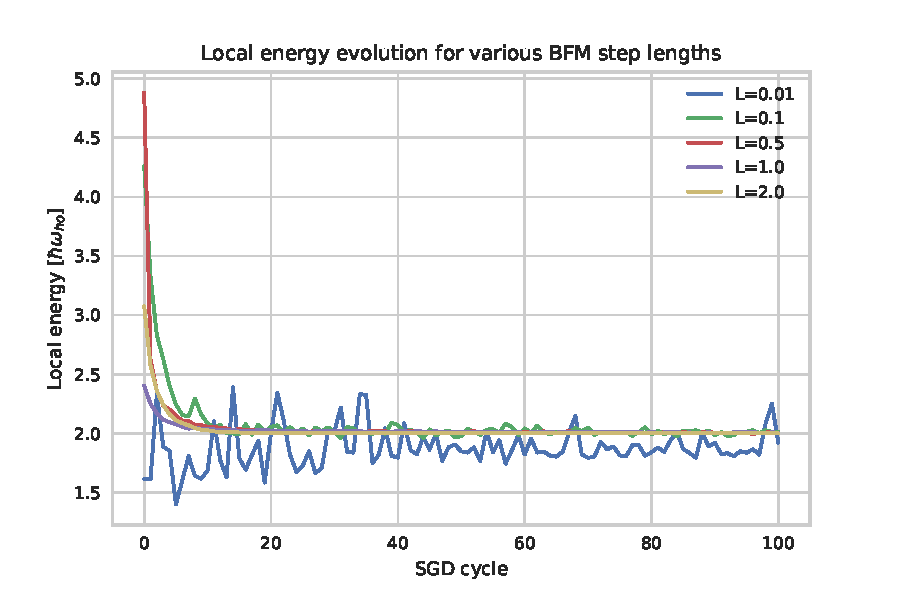
\includegraphics[scale=1.0]{plot1.pdf}
\caption{Local energy evolution calculated as the program adapts using Stochastic Gradient Descent for various Metropolis step lengths. Two particles in two dimensions with two hidden nodes and $\eta = 0.10$ are considered. We note how for $L\geq 0.5$ are quite stable at $E_L=2\ \hbar\omega_{ho}$.}
\label{Fig:1}
\end{figure}

As we can see from the figure, $L=0.01$ underestimates the correct value and the system does not equilibrate, $L=0.1$ oscillates around the correct value for a long time. On the other hand for $L\geq0.5$ equilibrium is reached after only a few cycles, which is desirable. Therefore it appears that a larger step length produces a faster equilibrium. This is reasonable: with a large step length we move more the particles at each step and thus even though we start with a bad configuration, we will reach faster a good one through the SGD. It appears that $L=1.0$ is the fastest one to converge. 
Moreover we study also the behaviour of the acceptance ratio of Monte Carlo steps as a function of the step length. The results are shown in Tab. (\ref{Tab:1}). We note that using a very large L results in a small acceptance ratio and by consequence we sample the same positions many times, effectively producing worse statistics. Therefore it is desirable to use a step length that results in a higher acceptance ratio. 

\begin{table}[H]
\caption{Acceptance ratio as function of BFM step length. The data are made using  2 particles in 2 dimensions with 2 hidden nodes.}
\centering
\begin{tabular}{c| c } 
\textbf{L} & \textbf{Acceptance ratio} \\ \hline
2.0  & 0.73   \\
1.0 & 0.85  \\
0.5  &  0.93 \\
0.1  &  0.985 \\
0.01  &  0.999 \\ 
\end{tabular}
\label{Tab:1}
\end{table} 

%Each SGD cycle notes the standard deviation of the local energy. 
In Fig. (\ref{Fig:2}) we study the evolution of the standard deviation computed through the blocking method (which takes into account correlations of data) of the local energy as the the SGD cycles advance. From the figure we can extract that by using small step length ($L=0.01,0.1$) the error is larger than the other cases and that the standard deviation undergoes large fluctuations. On the other hand for larger step length, the fluctuations as well as the errors decrease.

\begin{figure}[H]
	\centering
	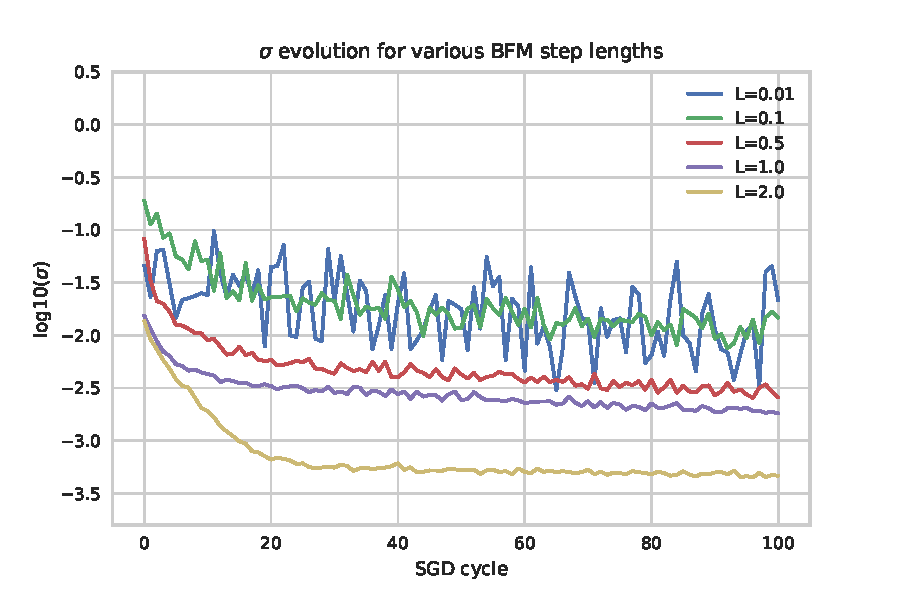
\includegraphics[scale=1.00]{plot2.pdf}
	\caption{Local energy evolution calculated as the program adapts using Stochastic Gradient Descent for various BFM step lengths. Two particles in two dimensions with two hidden nodes and $\eta = 0.10$ are considered. As we increase the BFM step length, the value of $\sigma$ as well as its fluctuation decrease with the exception of the first two step length.}
	\label{Fig:2}
\end{figure} 

By combining the data from Fig. (\ref{Fig:1}), Fig. (\ref{Fig:2}) and Tab. \ref{Tab:1}, we conclude that $L = 1.0$ is an appropriate choice of step length for the BFM algorithm. Also $L=0.5,2.0$ could be good choices, but $L=1.0$ is the most balanced one: it has a good acceptance ratio, low $\sigma$ and it is the fastest to converge.

To understand how the learning works and which is the best learning rate to use, we plot in Fig. (\ref{Fig:3}) the SGD energy optimization of the RBM applied to 2 bosons in 2D for multiple learning rates. The figure shows that small learning rates use a long time to converge. Learning rate $\eta=0.01$ does converge to the same value after approximately 100 SGD cycles, $\eta=0.05$ converges after 50 cycles and the others converge with less than 10 cycles. We verify that increasing $\eta$ beyond 0.6 results in a diverging energy. 

\begin{figure}[H]
\centering
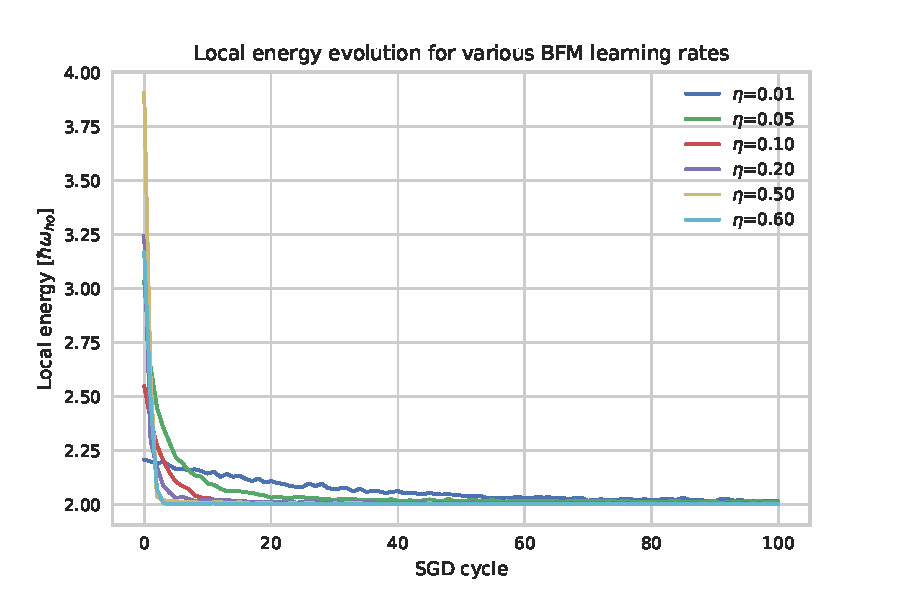
\includegraphics[scale=1.00]{plot3.pdf}
\caption{Local energy evolution calculated with BFM algorithm as the program adapts using SGD for two particles in 2D. BFM step length 1.0 is used for all the runs. Smaller learning rates give slower convergence.}
\label{Fig:3}
\end{figure}


\subsection{ISMH algorithm}

As we have done above with the BFM, we study the system with the Importance Sampling Metropolis-Hastings algorithm by taking into account its behaviour as we change the time step $\Delta t$. 

In Fig. (\ref{Fig:4}) is shows the SGD cycle energy adaption for multiple ISMH $\Delta t$. The data are made using $\eta = 0.10$. We can see that the velocity of convergence for $\Delta$ t $\in [0.001,2.00]$ is almost the same. However, in the case of $\Delta t=0.001$, the system does not converge well to the energy minimum: this is the only data series that visibly fluctuates. From this we can conclude that we should use $\Delta t > 0.001$. 

\begin{figure}[ht]
\centering
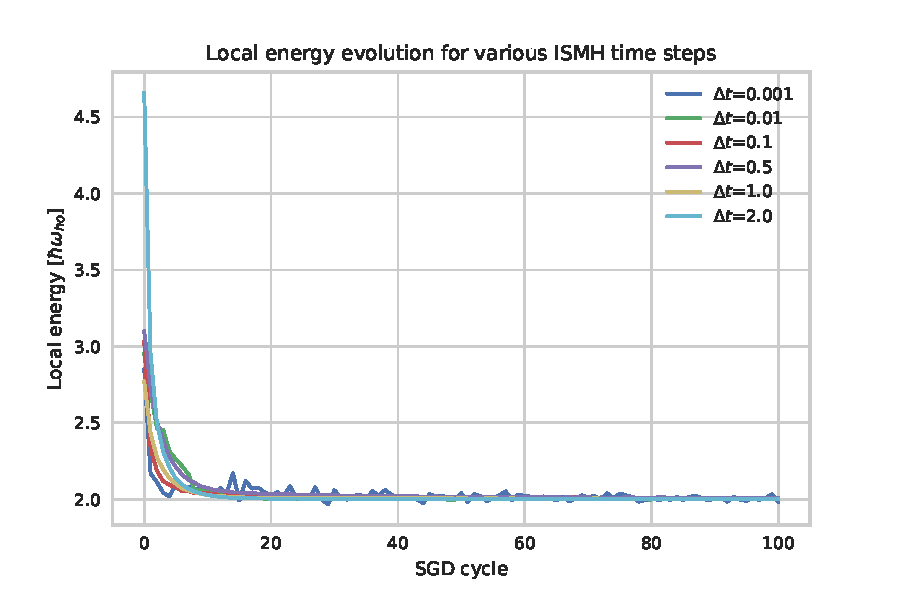
\includegraphics[scale=1.0]{plot4.pdf}
\caption{Local energy evolution calculated with ISMH algorithm as the program adapts using SGD for two particles in 2D. The data are made using $\eta = 0.10$ and 2 hidden nodes. The convergence time is very fast, and is almost independent of $\Delta t$. Using $\Delta t=0.50$ is faster than the other time steps. All the time steps converge to the same energy. Using $\Delta t = 0.001$, the local energy fluctuates visibly for 100 cycles. It will therefore be favorable to use $\Delta t > 0.001$.}
\label{Fig:4}
\end{figure}
At this point we plot (Fig. (\ref{Fig:5})) the logarithm of the standard deviation of the local energy of the data from Fig. (\ref{Fig:4}) as function of SGD cycles. The data show that by increasing the time step the $\sigma$ decreases even though for $\Delta t\in [1.0, 2.0]$ is almost the same. Moreover the standard deviation becomes smoother as the time step increases. 

\begin{figure}[H]
\centering
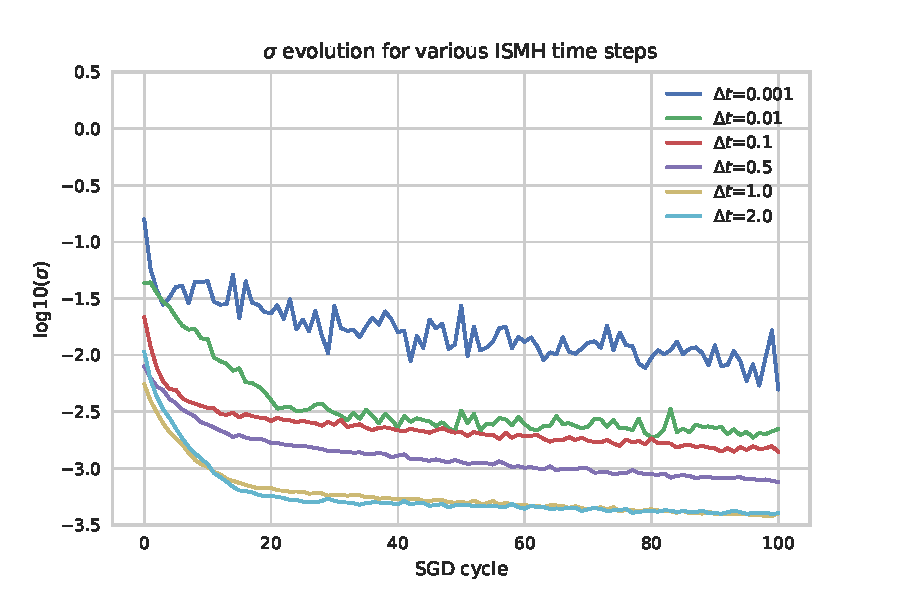
\includegraphics[scale=1.0]{plot5.pdf}
\caption{Logarithm of the standard deviation evolution calculated with ISMH algorithm as the program adapts using SGD for two particles in 2D. The data are made using $\eta = 0.1$. $\Delta t\leq 0.05$ use a long time to converge to the energy. It will therefore be favorable to use $\Delta t > 0.05$.}
\label{Fig:5}
\end{figure}
% 1.3.2 learn rate 0.1
In Tab. \ref{Tab:2} we show the acceptance rate of Monte Carlo steps using ISMH as a function of $\Delta t$. Again we wish to have a large acceptance ratio. This ratio should not be close to one, though.  In fact that would mean that we are accepting all the moves which is a signal that we are not moving enough the particles at each Monte Carlo step. From the table, the best option is obviously $\Delta t = 0.50$. 

\begin{table}[H]
\centering
\caption{Acceptance ratio as function of ISMH time step. The data are made using 2 particles in 2 dimensions and 2 hidden nodes.}
\begin{tabular}{c| c } 
\textbf{$\boldsymbol{\Delta}$t} & \textbf{Acceptance ratio} \\ \hline
2 & 0.49 \\
1 & 0.78 \\
0.5 & 0.92  \\
0.1  &  0.993 \\
0.05  &  0.997 \\
0.01  &  0.9998 \\
0.001 & 0.99999 \\ 
\end{tabular}
\label{Tab:2}
\end{table} 

By combining this with the considerations expressed above, we conclude $\Delta t= 0.50$ is an acceptable time step, it will be used in the further computations. 

As regards the learning rate, we note that varying $\eta$ (Fig. (\ref{Fig:6})) produces results similar to the ones of Fig. (\ref{Fig:3}): $\eta=0.01$ converges really slowly in about more than 100 cycles, whereas the other learning rates converges almost with the same speed.



\begin{figure}[H]
\centering
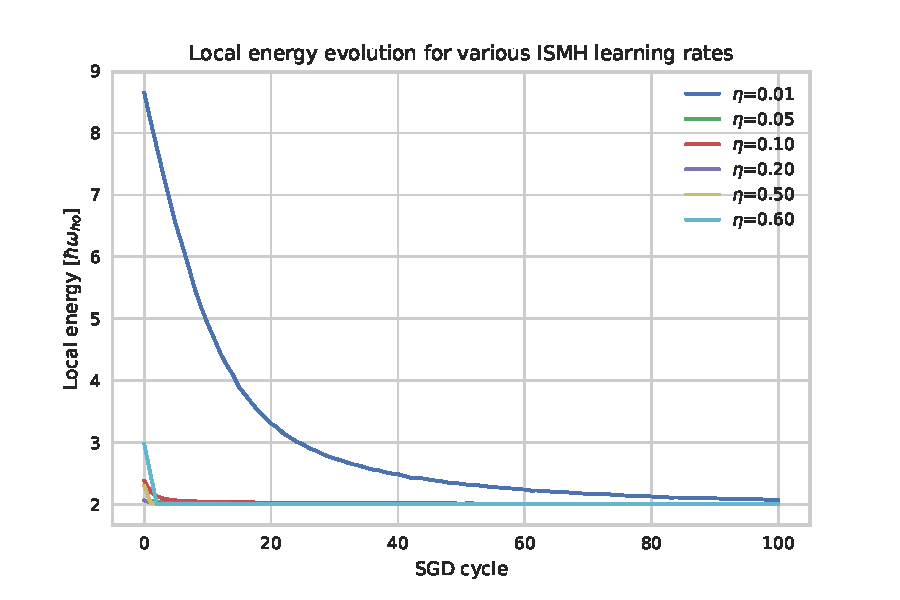
\includegraphics[scale=1.0]{plot6.pdf}
\caption{Local energy evolution calculated with ISMH algorithm sampling as the program adapts using SGD for two particles in 2D. Importance Sampling time step 0.5 is used for all the runs. Even though all the learning rates converge, we note that $\eta=0.01$ converges really slowly.}
\label{Fig:6}
\end{figure} 


\subsection{Energy of non-interacting bosons in a spherical harmonic trap}
Having found all the "right" parameters for each sampler, we proceed to give some values of energy for different configurations of particles, dimensions and number of hidden nodes. We use as learning rate $\eta=0.6$ because it seems the largest stable and we want the fastest convergence. After some running, we have understood that by increasing the number of hidden nodes and with D$=3$, the system gets more instable and thus we have to decrease the learning rate: we set $\eta=0.2$ when M$=4$ and $\eta=0.1$  when D$=3$.

In Tab. \ref{Tab:3} we show the ground state local energy of non-interacting bosons computed with the different samplers. Results regarding one and two particle in 1D and 2D agree really well with the analytical predictions. On the other hand, the agreement between the analytical results and the samplers data is not good. This might suggest that we should have used more cycles for the convergence. In general it appears ISMH produces smaller errors than BFM. For both algorithms the error increases as more hidden nodes are added.  

\begin{table}[H]
\centering
\caption{Local energy of non-interacting bosons in a spherical harmonic trap. The quantity $N_p$ is the number of bosons, D is the dimensionality, M is the number of hidden nodes and $\eta$ is the learning rate. We show the analytical results and the ones obtained with BFM as well as ISMH algorithms. The setup consists on 300 SGD cycles of 300 000 MC steps. The final run to compute the energy is done with $10^7$ MC steps. The BFM step length is $L=1.0$, ISMH time step is $\Delta t = 0.5$. Both algorithms use $\sigma = 1.00$.  The error is calculated using the blocking method.}
\begin{tabular}{c c c c |c c c} 
$\boldsymbol{N_p}$ & \textbf{D}  & $\boldsymbol{M}$ & $\eta$ & \textbf{Analytical} & \textbf{BFM} & \textbf{ISMH} \\
&&&&$[\hbar\omega_{ho}]$ &$[\hbar\omega_{ho}]$&$[\hbar\omega_{ho}]$\\\hline
1 & 1 & 1 & 0.6 & 0.5  & $\SI{0.50002\pm 0.00001}{}  $ & $\SI{0.500001\pm 0.000001}{}$ \\ \hline
1 & 2 & 1 &0.6 & 1.0   & $\SI{1.00003\pm 0.00002}{} $ & $\SI{1.000000\pm 0.000003}{}$ \\
1 & 2 & 2 &0.6 & 1.0   & $\SI{1.00003\pm 0.00002}{} $ & $\SI{1.00004\pm 0.00001}{}$ \\ \hline
1 & 3 & 1 &0.1 & 1.5  &  $\SI{1.5003\pm 0.0001}{} $ &  $\SI{1.50033\pm 0.00003}{}$\\
1 & 3 & 2 &0.1 & 1.5   &  $\SI{1.5005\pm 0.0001}{} $ & $\SI{1.50069\pm 0.00003}{}$ \\
1 & 3 & 3 &0.1 & 1.5   &  $\SI{1.5005\pm 0.0001}{}$&   $\SI{1.50058\pm 0.00003}{}$\\ \hline
2 & 1 & 1 &0.6 & 1.0  & $\SI{1.00006\pm 0.00002}{} $ & $\SI{1.00003\pm 0.00001}{}$ \\ 
2 & 1 & 2 &0.6 & 1.0  & $\SI{1.00003\pm 0.00001}{}$ & $\SI{1.00004\pm 0.00001}{}$ \\ \hline
2 & 2 & 1 &0.6 & 2.0  & $\SI{2.00009\pm 0.00003}{}$ & $\SI{2.00006\pm 0.00001}{}$ \\
2 & 2 & 2 &0.6 & 2.0   & $\SI{2.0002\pm 0.0003}{}$ & $\SI{2.00010\pm 0.00001}{}$ \\
2 & 2 & 3 &0.6 & 2.0   & $\SI{2.0001\pm 0.0004}{}$ & $\SI{2.00008\pm 0.00001}{}$ \\
2 & 2 & 4 &0.2 & 2.0   & $\SI{2.0007\pm 0.0001}{}$ & $\SI{2.00068\pm 0.00004}{}$ \\ \hline 
2 & 3 & 1 &0.1 & 3.0   &   $\SI{3.0012\pm 0.0002}{}$&  $\SI{3.0010\pm 0.0001}{}$ \\
2 & 3 & 2 &0.1 & 3.0   &   $\SI{3.0017\pm 0.0002}{}$&  $$\SI{3.0020\pm 0.0001}{}$$ \\
2 & 3 & 3 &0.1 & 3.0   &  $\SI{3.0026\pm 0.0003}{}$&    $\SI{3.0018\pm 0.0001}{}$ \\
2 & 3 & 4 &0.1 & 3.0   &  $\SI{3.0024\pm 0.0003}{}$&   $\SI{3.0036\pm 0.0001}{}$ \\
2 & 3 & 5 &0.1 & 3.0  &  $\SI{3.0036\pm 0.0003}{}$  &  $\SI{3.0039\pm 0.0001}{}$  \\
2 & 3 & 6 &0.1 & 3.0   &  $\SI{3.0044\pm 0.0003}{}$   & $\SI{3.0051\pm 0.0001}{}$  \\ 
\end{tabular}
\label{Tab:3}
\end{table} 

\section{Non-interacting bosons in an elliptical harmonic trap}
At this point, we change the shape of the harmonic trap: we consider the Hamiltonian in eq. (\ref{ham}). There are no reasons to think that the parameters found in the previous sections (such as BFM step length, ISMH time step) should change. Hence we use the same. Only the 3D case is involved in the change of symmetry since we modify the z direction. Therefore we focus our analysis on the 3D case. Again we only consider cases of one or two particles for computational speed. Nevertheless we decide to use the Importance Sampling Metropolis-Hastings algorithm since it has proved to be the one which gives smaller errors.  In Tab. (\ref{Tab:3.2}), we show the results obtained with the elliptical harmonic trap. In \cite{vmcarticle}, Dubois and Glyde show $E/N=2.414\ \hbar\omega_{ho}$ for this trap. As we can see from the table, the results are not compatible with the predictions for many standard deviations. This is unexpected. 

\begin{table}[H]
	\centering
	\caption{Local energy per particle $E_L/N_p$ of non-interacting bosons in an elliptical harmonic trap. The quantity $N_p$ is the number of bosons, D is the dimensionality, M is the number of hidden nodes and $\eta$ is the learning rate. We show the analytical results and the ones obtained with ISMH algorithm. The setup consists on 300 SGD cycles of 300 000 MC steps. The final run to compute the energy is done with $10^7$ MC steps. The ISMH time step is $\Delta t = 0.5$ and $\sigma = 1.00$.  The error is calculated using the blocking method.}
	\begin{tabular}{c c c c |c  c} 
		$\boldsymbol{N_p}$ & \textbf{D}  & $\boldsymbol{M}$ & $\eta$ & \textbf{Analytical} &\textbf{ISMH} \\
		&&&&$[\hbar\omega_{ho}]$ &$[\hbar\omega_{ho}]$\\\hline
		1 & 3 & 1 &0.1 &           2.414                &          $\SI{3.247\pm 0.002}{}$              \\
		1 & 3 & 2 &0.1 &           2.414                 &       $\SI{3.250\pm 0.002}{}$                 \\
		1 & 3 & 3 &0.1 &           2.414                 &       $\SI{3.251\pm 0.002}{}$                 \\ \hline
		2 & 3 & 1 &0.1 &           2.414                 &      $\SI{3.25\pm 0.01}{}$                  \\
		2 & 3 & 2 &0.1 &           2.414                 &      $\SI{3.25\pm 0.01}{}$                  \\
		2 & 3 & 3 &0.1 &           2.414                 &      $\SI{3.25\pm 0.01}{}$                 \\
		2 & 3 & 4 &0.05 &           2.414                 &      $\SI{3.26\pm 0.01}{}$            \\
		2 & 3 & 5 &0.05&            2.414                &      $\SI{3.25\pm 0.01}{}$                  \\
		2 & 3 & 6 &0.05 &           2.414                 &      $\SI{3.25\pm 0.01}{}$                  \\ 
	\end{tabular}
	\label{Tab:3.2}
\end{table} 

%	1 & 3 & 1 &0.1 &           2.414                &          $3.247\pm 0.002$              \\
%	1 & 3 & 2 &0.1 &           2.414                 &       $3.250\pm 0.002$                 \\
%	1 & 3 & 3 &0.1 &           2.414                 &       $3.251\pm 0.002$                 \\ \hline
%	2 & 3 & 1 &0.1 &           4.828                 &      $6.496\pm 0.005$                  \\
%	2 & 3 & 2 &0.1 &           4.828                 &      $6.502\pm 0.005$                  \\
%	2 & 3 & 3 &0.1 &           4.828                 &      $6.500\pm 0.005$                  \\
%	2 & 3 & 4 &0.05 &           4.828                 &      $6.508\pm 0.005$            \\
%	2 & 3 & 5 &0.05&            4.828                &      $6.496\pm 0.005$                  \\
%	2 & 3 & 6 &0.05 &           4.828                 &      $6.501\pm 0.005$       
%  

%\section{Interacting Bosons in an elliptic harmonic trap}
%After having implemented the Hamiltonian in eq. (\ref{eq_hamilton}) with the elliptical harmonic trap, it has been immediately clear that with the actual trial wave-function something was wrong. The data obtained with $10$ particles in 3 dimensions with various number of hidden nodes were too high: the energy was about $\sim 3.3$ per particle instead of something around $\sim 2.4$ as \cite{DalfString}. There are a number of reasons which made us believe that there is something "weird" as regards these results:
%\begin{enumerate}
%	\item in a project made before were we studied this Hamiltonian with a different trial wave-function using the so-called Variational Monte-Carlo (VMC), we obtain with good precision $2.414$ for one particle. 
%	\item In the non-interacting case we obtain results compatible with the analytical ones with really good precision. Here we are basically just changing the shape of the harmonic potential from spherical to elliptical.
%\end{enumerate} 
A possible conclusion could be that our RBM does not learn the elliptical symmetry given by the harmonic potential in a reasonable amount of time. In principle the symmetry should be learned in an infinitive time, we do not have such time, therefore we try to fix this problem by enhancing the importance of the z-ax. Our ansatz is that this enhancement should be a certain combination of $\lambda$ that we call $\xi$. Moreover we guess that there is an appropriate value of $\xi$ for the nodes in the z direction ($\xi_1$) as well as one appropriate for the biases $w_{ij}$ which involve the z direction ($\xi_2$). We insert a $\xi_1$ each time we find a $X_i$ and a $\xi_2$ each time we have $w_{ij}$. The enhancement is activated only when the z-ax is considered. The trial wave-function becomes

\begin{equation*}
	\label{new_trial_wf}
	\Psi(\mathbf{X}) = \frac{1}{Z} \exp\bigg[-\sum_i^M \frac{(X_i\xi_1-a_i)^2}{2\sigma^2}\bigg]\prod_j^N \left(  1 + \exp\bigg[b_j +\sum_i^M \frac{X_i\ \xi_1\ w_{ij}\ \xi_2}{\sigma^2}\bigg]\right)	
\end{equation*}

By trials and errors, ww try to find the good values of $\xi_1$ and $\xi_2$ that match our theoretical prediction. However, the system seems to be less stable than before. For this reason, we have to lower the learning rate and to increase the number of SGD cycles to 600. Anyway, the system does not converge precisely to a value but it oscillates. Hence, to give a value of energy, we average the energies given by each cycle after the system has equilibrated. We find that values of 
\begin{equation*}
	\xi_1=\sqrt[4]{\lambda}\qquad \xi_2=\lambda^2
\end{equation*}
give the results in Tab. (\ref{Tab:3.3}). The results are compatible with the analytical ones with $3\sigma$. Overall it seems that we overestimate the analytical values. Nevertheless we decide to use this setup for our computations.  

\begin{table}[H]
	\centering
	\caption{Local energy per particle $E_L/N_p$ of non-interacting bosons in an elliptical harmonic trap where $\Psi$ is fixed with $\xi_1$ and $\xi_2$. The quantity $N_p$ is the number of bosons, D is the dimensionality, M is the number of hidden nodes and $\eta$ is the learning rate. We show the analytical results and the ones obtained with ISMH algorithm. The setup consists on 600 SGD cycles of 300 000 MC steps. The ISMH time step is $\Delta t = 0.5$ and $\sigma = 1.00$.  The error is calculated using the blocking method.}
	\begin{tabular}{c c c c |c  c} 
		$\boldsymbol{N_p}$ & \textbf{D}  & $\boldsymbol{M}$ & $\boldsymbol{\eta}$ & \textbf{Analytical} &\textbf{ISMH} \\
		&&&&$[\hbar\omega_{ho}]$ &$[\hbar\omega_{ho}]$\\\hline
		1 & 3 & 1 &0.1 &           2.414                &        $\SI{2.44\pm 0.01}{}$                \\
		1 & 3 & 2 &0.1 &           2.414                 &     $\SI{2.44\pm 0.01}{}$                   \\
		1 & 3 & 3 &0.05 &           2.414                 &     $\SI{2.44\pm 0.01}{}$                   \\ \hline
		2 & 3 & 1 &0.05 &           2.414                 &     $\SI{2.44\pm 0.01}{}$                   \\
		2 & 3 & 2 &0.01 &           2.414                 &     $\SI{2.44\pm 0.01}{}$                   \\
		2 & 3 & 3 &0.01 &           2.414                 &      $\SI{2.44\pm 0.01}{}$                  \\
		2 & 3 & 4 &0.01 &           2.414                 &     $\SI{2.44\pm 0.01}{}$                   \\
		2 & 3 & 5 &0.01 &            2.414                &  $\SI{2.44\pm 0.01}{}$                            \\
		2 & 3 & 6 &0.01 &           2.414                 &   $\SI{2.44\pm 0.01}{}$                           \\ 
	\end{tabular}
	\label{Tab:3.3}
\end{table} 